\documentclass[12pt, letterpaper]{article}
\usepackage{graphicx} %LaTeX package to import graphics
\graphicspath{{images/}} %configuring the graphicx package
\usepackage{amsmath}
\title{Statistical Inference in HEP Assignments}
\author{Debaditya Chakrabarti, 20252021}
\begin{document}
\maketitle
\paragraph{Problem 1}
 Calculate mean and variance of a random number distributed according to the Chi2 pdf. 
\paragraph{Solution:}
The Chi Square pdf is given by:
\[ f(z; n) = \frac{z^{\frac{n}{2}-1} e^{-\frac{z}{2}}}{2^{\frac{n}{2}} \Gamma\left(\frac{n}{2}\right)} \quad \text{for } z > 0 \]

Gamma function is:
\[ \Gamma(n) = \int_0^\infty z^{n-1} e^{-z} dz \quad \text{for } n > 0 \]

We can write the "general" form of a Gamma function as:
\[ \frac{\Gamma(n)}{a^{n}} = \int_0^\infty z^{n-1} e^{-az} dz \]

Now we do a variable transformation to replace $n-1$ with $\frac{n'}{2}$ and replace $a$ with $\frac{1}{2}$. Upon doing so our new gamma function yields:
\[ \frac{\Gamma(\frac{n'}{2}+1)}{\left(\frac{1}{2}\right)^{\frac{n'}{2}+1}} = \int_0^\infty z^{\frac{n'}{2}} e^{-\frac{z}{2}} dz \]

For any continuious r.v $X$, the expectation value is defined by:
\[ E[X] = \int_{defined \hspace{1mm} region}^{} x f(x) dx \]

Now our expectation in this case resembles:
\[ E[z] = \int_{0}^{\infty} z \hspace{1mm} \frac{z^{\frac{n}{2}-1} e^{-\frac{z}{2}}}{2^{\frac{n}{2}} \Gamma\left(\frac{n}{2}\right)} dz \]
\[   = \int_{0}^{\infty} \frac{z^{\frac{n}{2}} e^{-\frac{z}{2}}}{2^{\frac{n}{2}} \Gamma\left(\frac{n}{2}\right)} dz \]
\[   = \frac{\int_{0}^{\infty} z^{\frac{n}{2}} e^{-\frac{z}{2}} dz }{{2^{\frac{n}{2}} \Gamma\left(\frac{n}{2}\right)}} \]
So we now replace the general integral which we had evaluated earlier with the new integral we have here. This yields:
\[ E[z]  = \frac{\frac{\Gamma(\frac{n'}{2}+1)}{\left(\frac{1}{2}\right)^{\frac{n'}{2}+1}}}{{2^{\frac{n}{2}} \Gamma\left(\frac{n}{2}\right)}} \]

Now cancelling a few terms using the identity $\Gamma(n+1) = n \Gamma(n)$ we get:
\[ E[z]=n\]

The variance is defined as:
\[ Var[X]=\int_{defined \hspace{1mm} region}^{} (x - E[X])^2 f(x) dx \]

Here we can replace $E[X]$ with $n$ and $f(x)$ with the Chi2 pdf. This yields:
\[ Var[X]=\int_{defined \hspace{1mm} region}^{} (x^{2} -2nx + n^2) f(x) dx \]
If we focus on the 2nd term of the integral, we can see that it is equal to $2nE[X]$ which is equal to $2n^2$. The 3rd term of the integral is equal to $n^2$ since the integral of a pdf over its defined region is equal to 1. The first term of the integral is equal to $E[X^2]$. So we can rewrite the variance as:
\[ Var[X] = E[X^2] - 2n^2 + n^2 \]
\[ Var[X] = E[X^2] - n^2 \]
We can calculate $E[z^2]$ from the "general" form of the gamma function we had derived earlier. We can replace $n-1$ with $\frac{n'}{2}+1$ and replace $a$ with $\frac{1}{2}$. Upon doing so our new gamma function yields:
\[ \frac{\Gamma(\frac{n'}{2}+2)}{\left(\frac{1}{2}\right)^{\frac{n'}{2}+2}} = \int_0^\infty z^{\frac{n'}{2}+1} e^{-\frac{z}{2}} dz \]. Dividing  this by our normalization consatnat namely: $2^{\frac{n}{2}} \Gamma\left(\frac{n}{2}\right)$ we get:
\[ E[z^2]= n^2+2n \] 
Now combining all integrals we get:
\[ Var[z] = E[z^2] - n^2 \]
\[ Var[z] = n^2+2n - n^2 \]
\[ Var[z] = 2n \]

\paragraph{Problem 2}
Take a dataset of your choice, sample various measurements under the assumption that each follow a gaussian profile to simulate 1000 experiments, and make a distribution of Chi2 (i.e. sum of square of deviations from the theory expectations weighed by respective uncertatinties). Study this for a few choices of ndofs.  Compare with Chi2 pdf of the same number of degrees of freedom.
\paragraph{Solution}
This exercise can be done either by generating a random set of datapoints or picking out an available dataset related to some phenomena. A few points from this dataset are sampled using
arbitrary algorithms, then these points can be chosen as mean and a Gaussian distribution with a given $\sigma$ can be generated from them. Now these set of distributions should be standerdized using the formula: $\frac{(X-\mu)}{\sigma}$.
After standardization we can sum up these r.v.s with a fixed mean to get our chi square distribution. The number of datapoints sampled or the number of standardized r.v.s added up are reffered to as the Degrees of freedom(dofs) of the system.
We hope that with increasing dofs Chi square will become Normal distribution because of central limit theorem.

\begin{figure}[htbp]
    \centering
    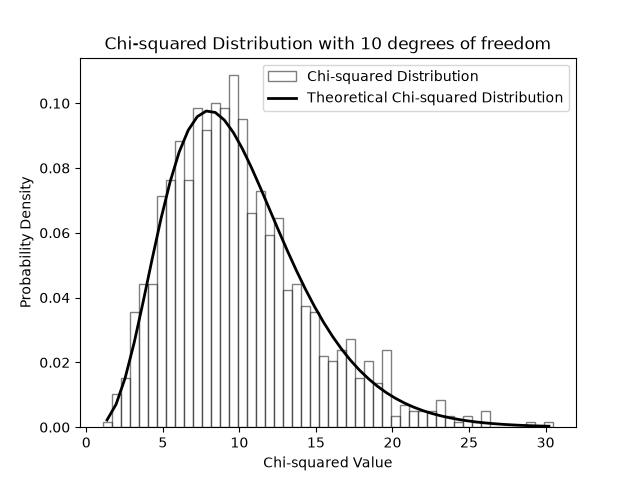
\includegraphics[width=1\textwidth]{Normal_Chi_Dof10.jpg}
\end{figure}

\begin{figure}[htbp]
    \centering
    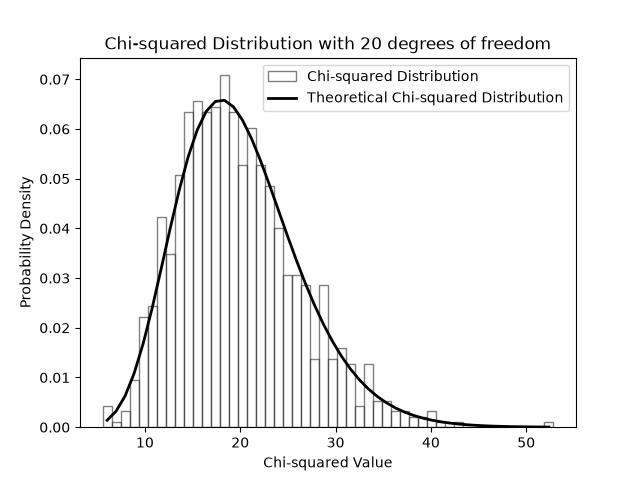
\includegraphics[width=1\textwidth]{Normal_Chi_Dof20.jpg}
\end{figure}

\begin{figure}[htbp]
    \centering
    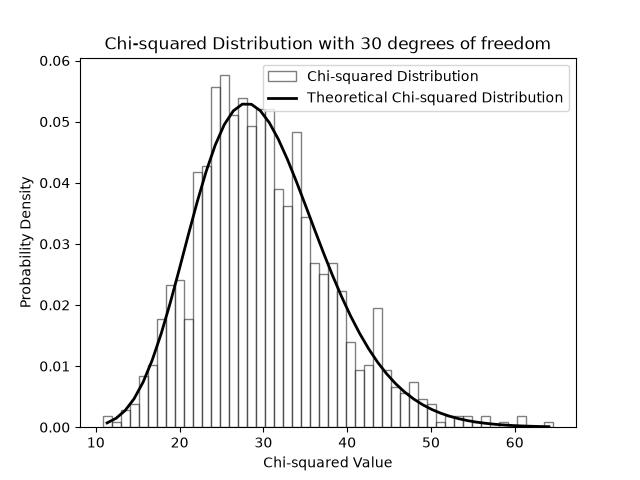
\includegraphics[width=1\textwidth]{Normal_Chi_Dof30.jpg}
\end{figure}

\begin{figure}[htbp]
    \centering
    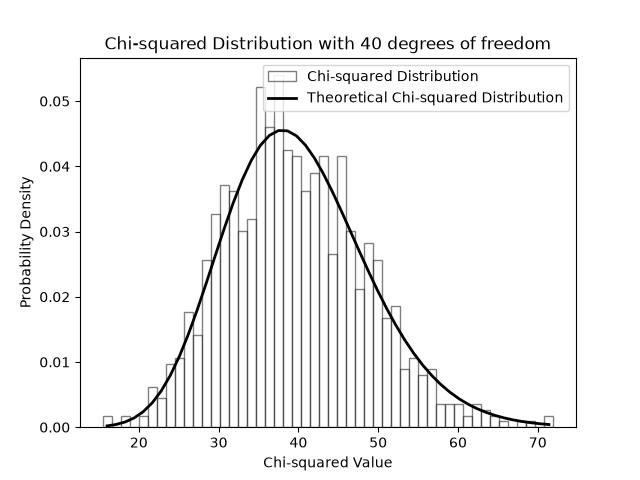
\includegraphics[width=1\textwidth]{Normal_Chi_Dof40.jpg}
\end{figure}

\newpage
\paragraph{Problem 3}
(3) Repeat (2) assuming non-Gaussian measurements.
\paragraph{Solution}
Here we did this for exponential and lognormal distributions. The steps are the same as the previous ones
except for the standardization part, for exponential the mean and standard deviation is the same on the other hand 
for log normal we need to take the logarithm of the r.v. A Chi square distribution is defined as the sum of standardized 
Gaussian i.i.ds(independent and identically distributed). So we don't expect them to match with the Chi square even with large degrees of freedom.


\begin{figure}[htbp]
    \centering
    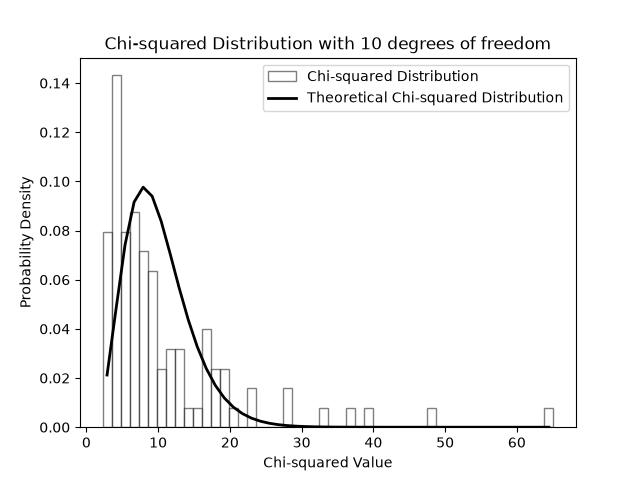
\includegraphics[width=1\textwidth]{Expo_Chi_Dof10.jpg}
\end{figure}

\begin{figure}[htbp]
    \centering
    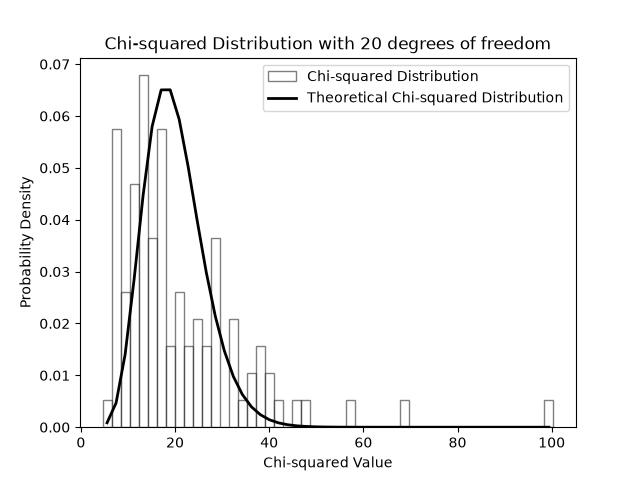
\includegraphics[width=1\textwidth]{Expo_Chi_Dof20.jpg}
\end{figure}

\begin{figure}[htbp]
    \centering
    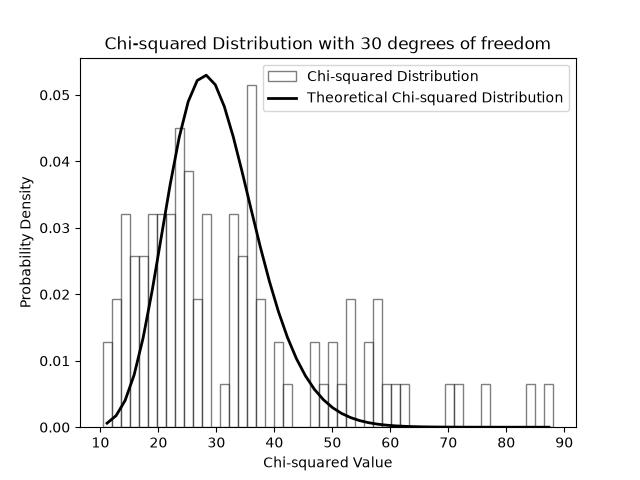
\includegraphics[width=1\textwidth]{Expo_Chi_Dof30.jpg}
\end{figure}

\begin{figure}[htbp]
    \centering
    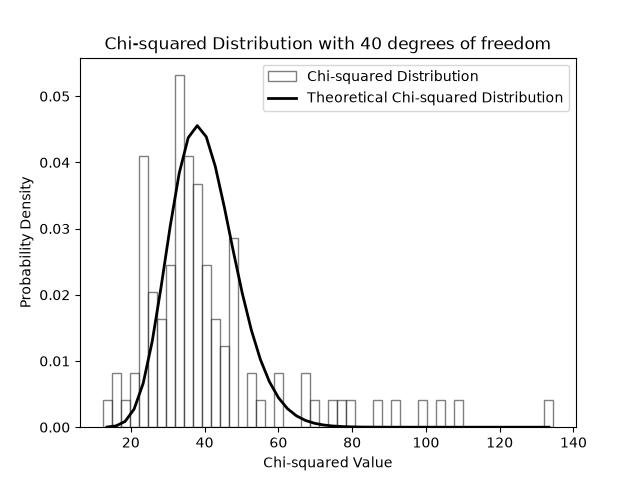
\includegraphics[width=1\textwidth]{Expo_Chi_Dof40.jpg}
\end{figure}
\newpage
All the above plots are for Exponential to Chisquare distribution

\begin{figure}[htbp]
    \centering
    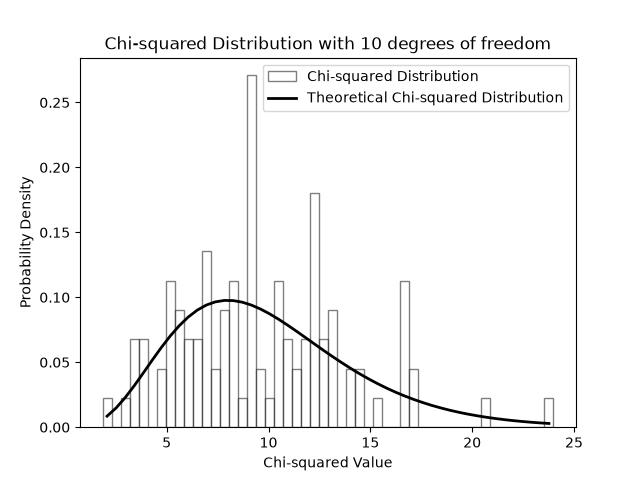
\includegraphics[width=1\textwidth]{Lognorm_Chi_Dof10.jpg}
\end{figure}

\begin{figure}[htbp]
    \centering
    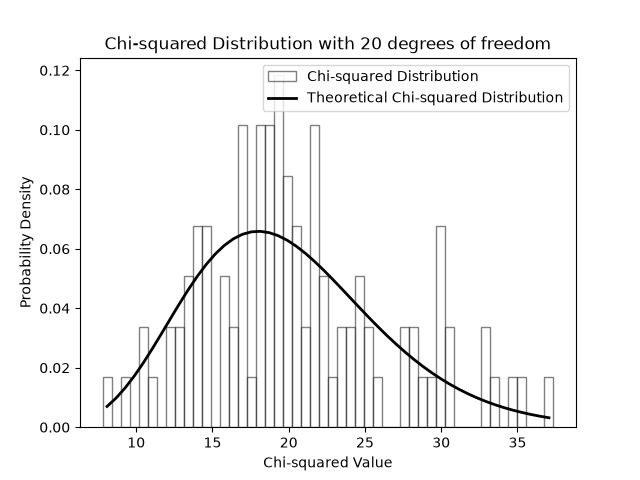
\includegraphics[width=1\textwidth]{Lognorm_Chi_Dof20.jpg}
\end{figure}

\begin{figure}[htbp]
    \centering
    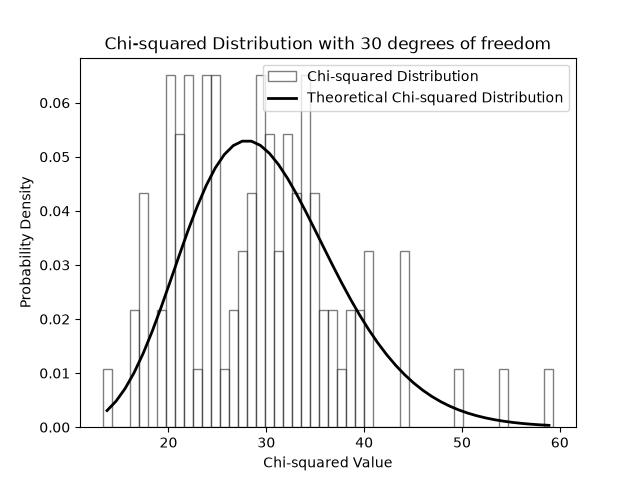
\includegraphics[width=1\textwidth]{Lognorm_Chi_Dof30.jpg}
\end{figure}

\begin{figure}[htbp]
    \centering
    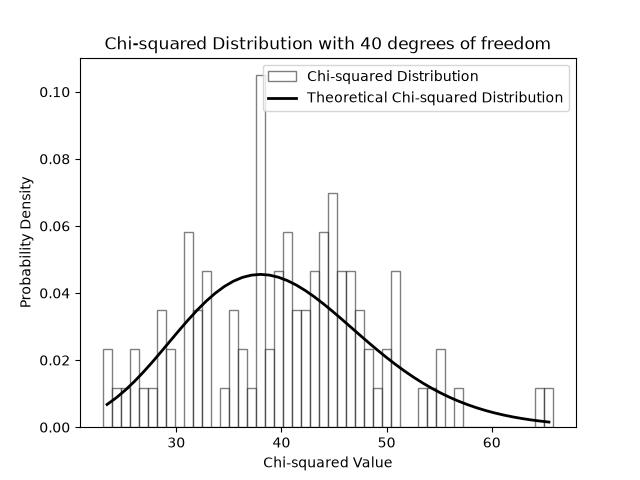
\includegraphics[width=1\textwidth]{Lognorm_Chi_Dof40.jpg}
\end{figure}
\newpage
All of the above are for Lognormal to Chi square.

\paragraph{Problem 4}
(4) Do a likelihood scan of pdf parameters to some data of your choice and verify that the value of likelihood or log-likelihood is maximum at the expected correct parameter values from which the dataset is sampled.
\paragraph{Solution:}
Here a data of normally distributed datapoints are used with true mean 0 and standarad deviation 0.5. 
We first scan for the mean in the range -1 to 1 and try to find the maximum of Loglikelihood function
defined by: $ln L(\mu, \sigma^2) = -\frac{n}{2} \ln(2\pi \sigma^2) - \frac{1}{2\sigma^2} \sum_{i=1}^{n} (x_i - \mu)^2 $ where n is the number of samples $\mu$ is mean and $\sigma$ is standard deviation.
The plot below shows our scan for mean:
\begin{figure}[htbp]
    \centering
    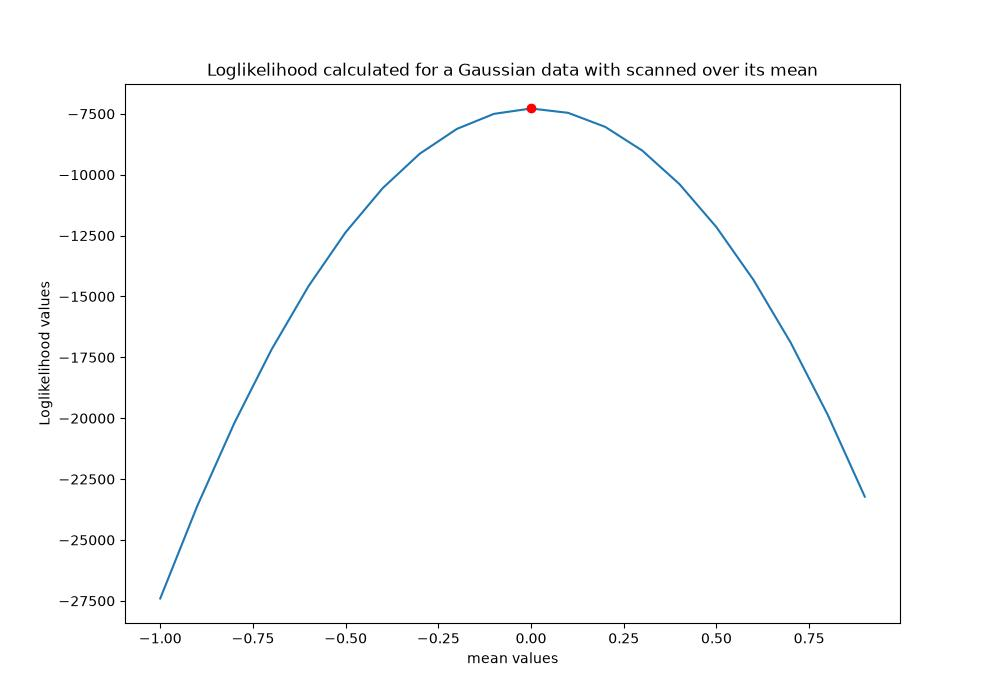
\includegraphics[width=1\textwidth]{MaximalLikelihoodformean.jpg}
\end{figure}
\newpage
Below one is for Standard Deviation:
\begin{figure}[htbp]
    \centering
    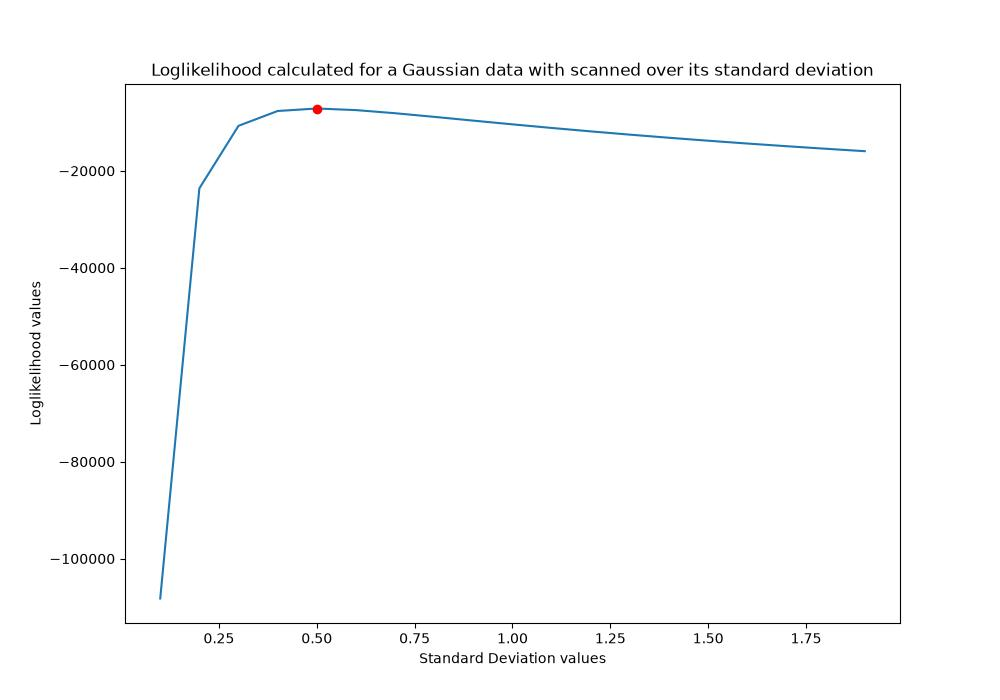
\includegraphics[width=1\textwidth]{MaximalLikelihoodforstd.jpg}
\end{figure}




\end{document}
